\section*{2. Hertzsprung-Russell diagram}

The table shows the effective temperature ($T_{eff}$), the absolute magnitude in the band $V$ ($M_V$),
and the bolometric correction ($BC$) for a group of stars.\\
\\
a) Using the data from the table below, plot the Hertzsprung-Russell diagram for the main-sequence stars
in terms of $M_V$ versus $log(T_{eff})$.\\
\\
b) Plot in the same diagram the curve that describes the stars with radii $R = 0.1$, $1.0$ and 
$10.0 R_\circ$. You can use that 
$L = 4 \pi R^2 \sigma T^4_{eff}$; $M_V + BC = M_{bol \circ} - 2.5 log(\frac{L}{L_\circ})$ where 
$M_{bol \circ} = + 4.74$ to derive the equation for the curve.\\
\\
\begin{center}
  \begin{tabular}{||c|c|c|c||c|c|c|c||}
        \hline
    S.N & $T_{eff}$ & $M_V$ & $BC$ & S.N & $T_{eff}$ & $M_V$ & $BC$\\
        \hline
    1 & 52500 & -6.0 & -4.751 & 15 & 6400 & 3.5 & -0.14\\
    2 & 44500 & -5.7 & -4.40 & 16 & 6200 & 4.0 & -0.16\\
    3 & 41000 & -5.5 & -3.93 & 17 & 6000 & 4.4 & -0.18\\
    4 & 35800 & -4.9 & -3.54 & 18 & 5800 & 4.7 & -0.20\\
    5 & 30000 & -4.0 & -3.16 & 19 & 5700 & 5.1 & -0.21\\
    6 & 18700 & -1.6 & -1.94 & 20 & 5600 & 5.5 & -0.40\\
    7 & 15400 & -1.2 & -1.46 & 21 & 5300 & 5.9 & -0.31\\
    8 & 11900 & -0.2 & -0.80 & 22 & 4900 & 6.4 & -0.42\\
    9 & 9500 & 0.6 & -0.30 & 23 & 4400 & 7.4 & -0.72\\
    10 & 8700 & 1.5 & -0.17 & 24 & 4100 & 8.1 & -1.01\\
    11 & 8200 & 1.9 & -0.15 & 25 & 3800 & 8.8 & -1.38\\
    12 & 7600 & 2.4 & -0.10 & 26 & 3600 & 9.9 & -1.89\\
    13 & 7200 & 2.7 & -0.09 & 27 & 3200 & 12.3 & -2.73\\
    14 & 6900 & 3.6 & -0.11 & 28 & 3100 & 13.5 & -3.21\\
        \hline
    \end{tabular}
\end{center}

\noindent\makebox[\textwidth]{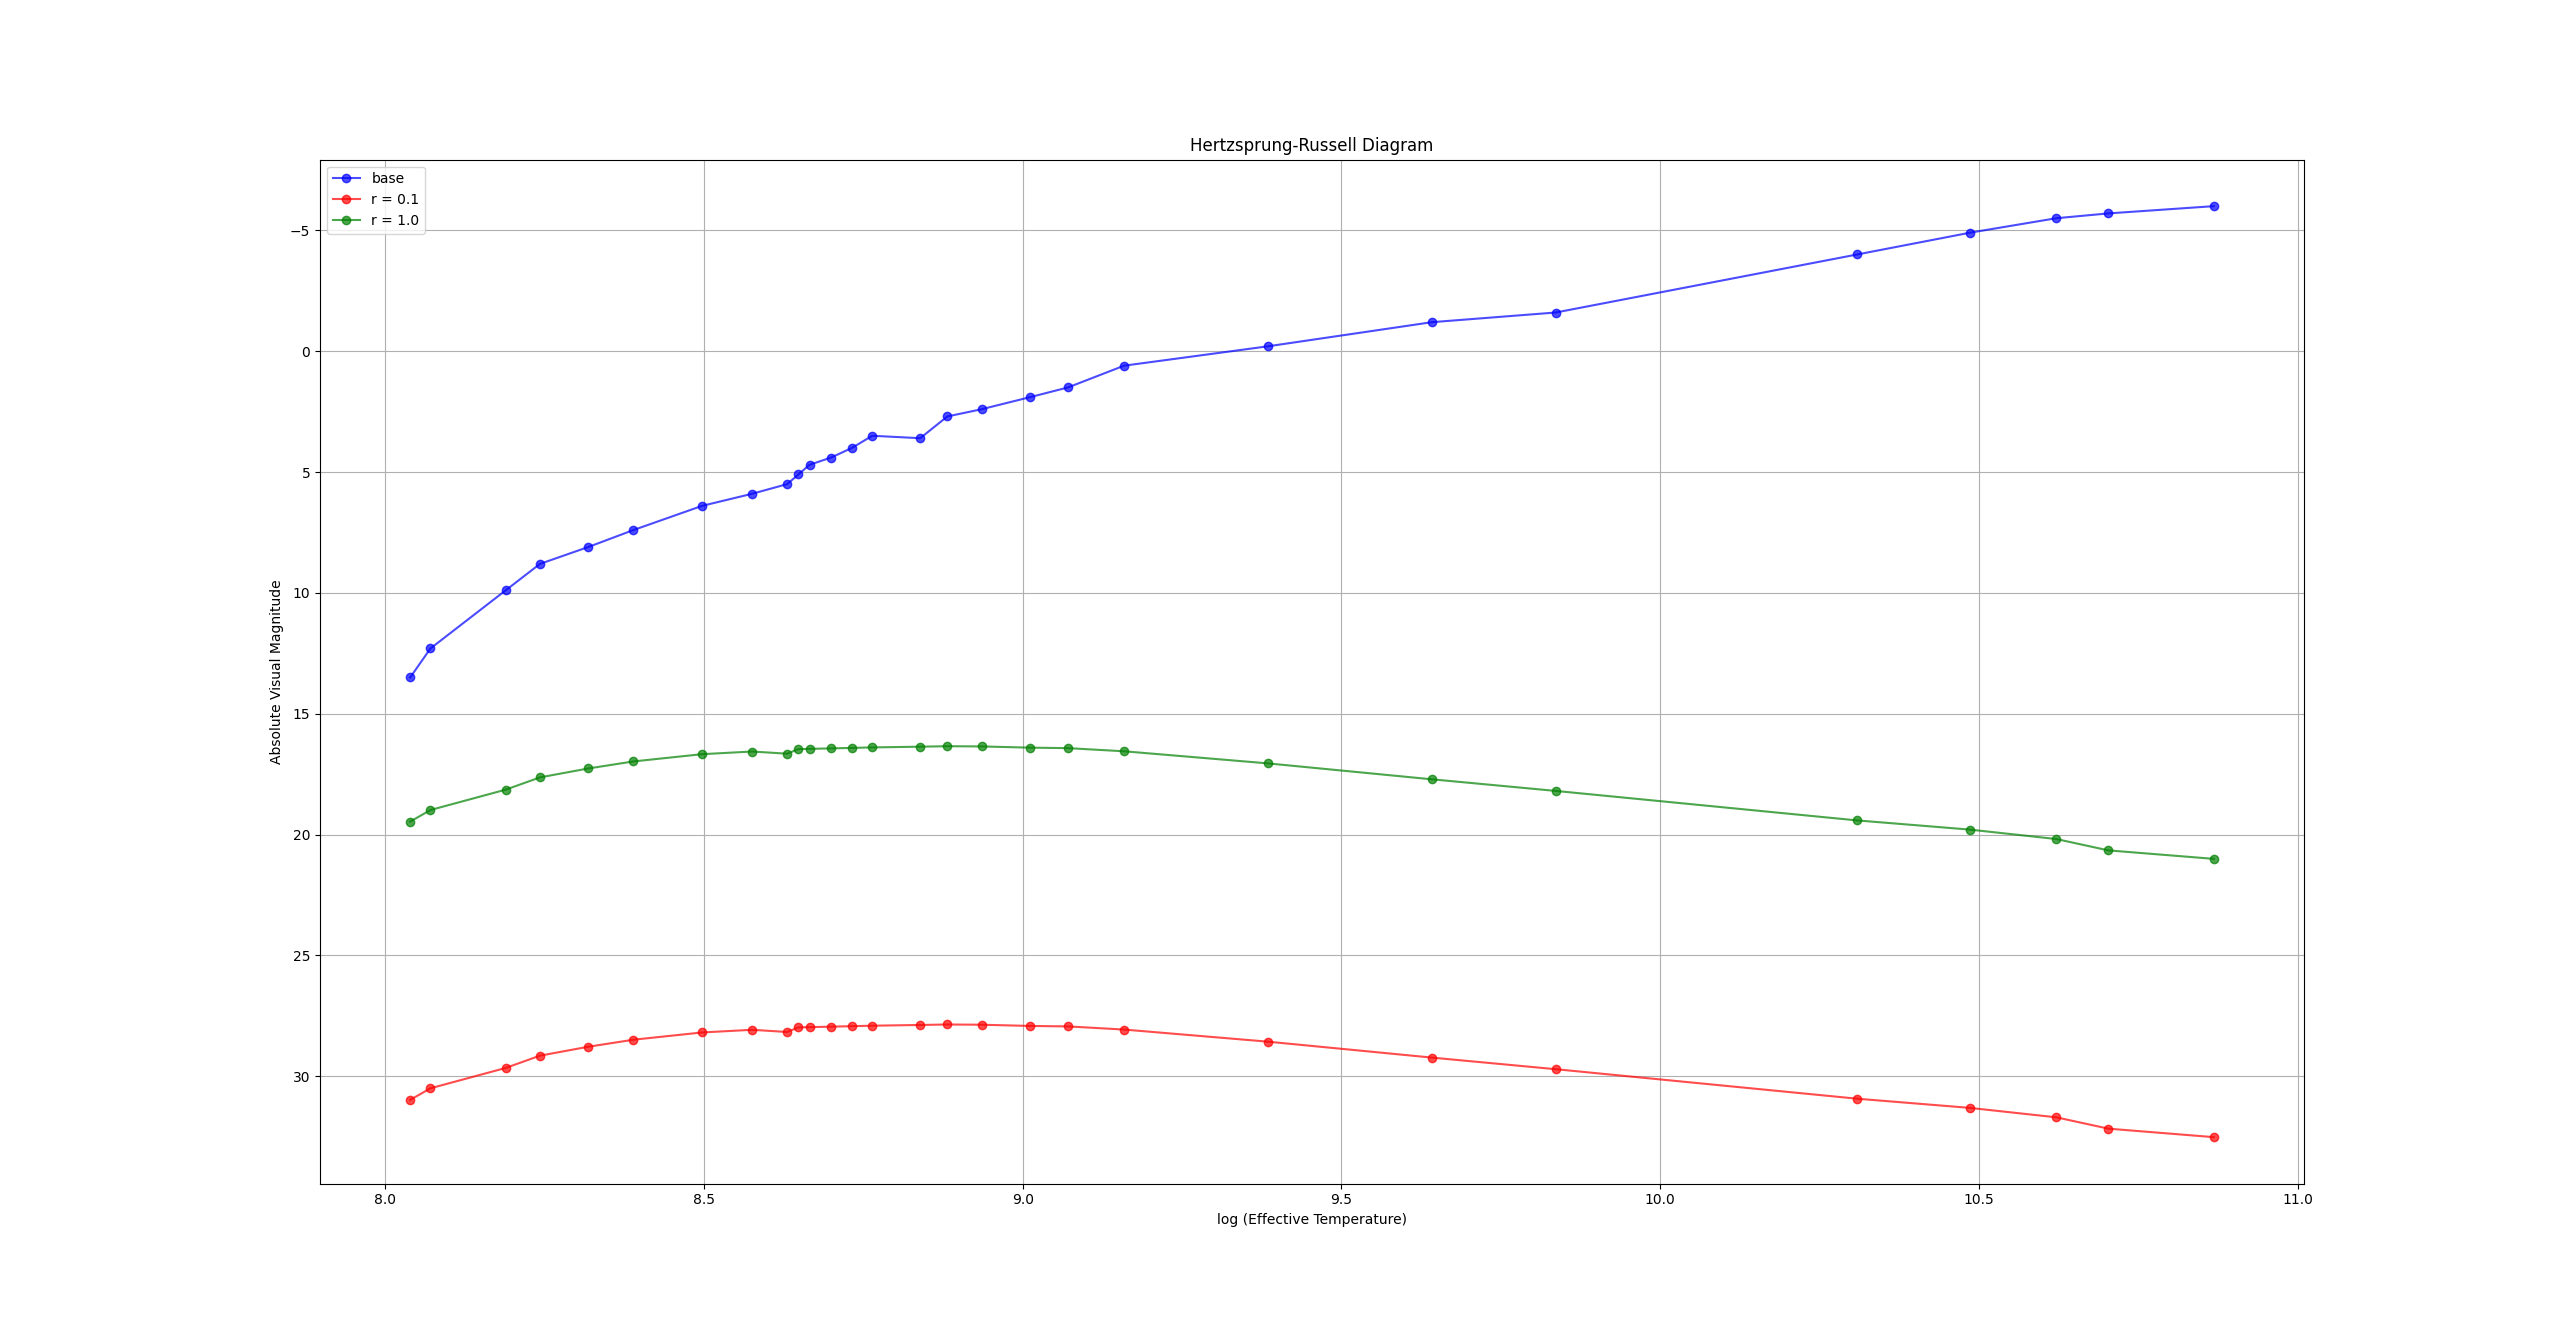
\includegraphics[scale=0.35]{russell.png}}\\
